\documentclass{article}
\usepackage{graphicx}
\usepackage{listings}
\usepackage{flexisym}

\graphicspath{ {images/} }

\newcommand{\overbar}[1]{\mkern 1.5mu\overline{\mkern-1.5mu#1\mkern-1.5mu}\mkern 1.5mu}

\begin{document}

  \title{CS 321: Assignment 5}
  \author{Jared Wasinger}

  \maketitle

	\begin{enumerate}
		\item\begin{enumerate}
			\item\begin{enumerate}
				\item Adversary picks $p$
				\item I pick: $w$ = $a^pb^{p+1}$\\
				\item Adversary splits $w$ into $w=xyz$
					\begin{itemize}
						\item $xy = a^{p}$ 
						\item$z=b^{p+1}$
						\item$|xy| \leq p$
						\item$|z| = p+1 > 0$
					\end{itemize}
			  \item I choose $i = 2$\\
					then, $xy^iz = xyyz$ has $p + |y|$ a's and p+1 b's.\\
					$p+2|y| > p+1$.  Therefore the number of a's is greater than b's.  $num(aa,w) \neq num(bbb,w)$. Thus, this language is not regular.
				\end{enumerate}
			\item\begin{enumerate}
				\item I choose $w = a^{p^2} \geq p$
				\item adversary splits $w$ into $xyz$\\
					$|xy| = p, |z| = p^2 - p > 0, |y| \geq p - 1$\\
					$|xz| = (p^2 - p) + (p - 1)$\\
				\item $p^2 - 1 \neq p^2$
				\item Proof by contradiction.  The language is not regular.
				\end{enumerate}
			\end{enumerate}
		\item\begin{enumerate}
		  \item 
				All strings where $\overbar{W} = rev(W)$  follow format:\\
				$SubStr.ReversedSubStr$\\
				CFG:\\
				$S \rightarrow 0S1 | 1S0 | \epsilon$
			\item 
				%$aSb \rightarrow aaSbb \rightarrow aabSabb$\\
				\textbf{Answer:} $S \rightarrow aSb | bSa | SS | \epsilon$\\
			\end{enumerate}
		\item $\{ w \in \{a,b\}^* | num(aaa,w) = num(bb,w)\}$\\
			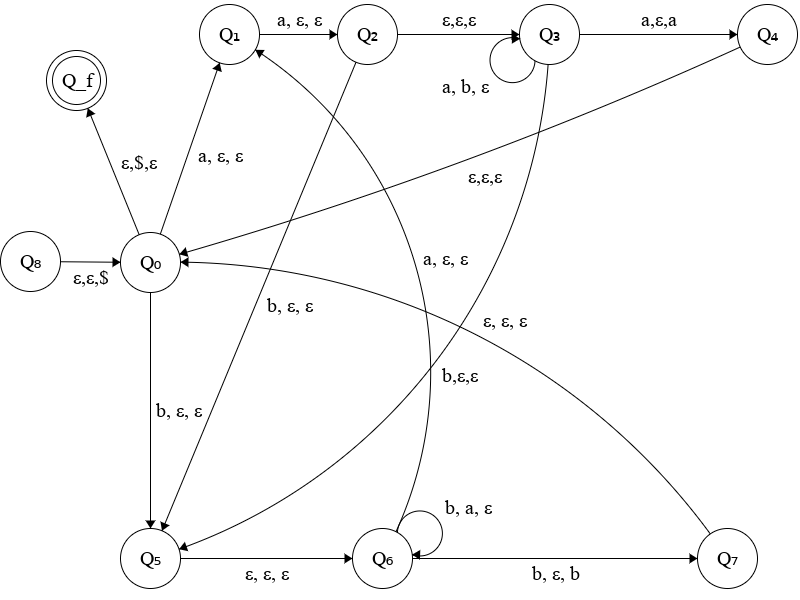
\includegraphics[width=\textwidth]{p3.png}\\
			\textbf{Explanation:}\\
				\begin{enumerate}
					\item The PDA starts out in state $Q_8$, pushing \$ onto the stack and moving to $Q_0$.
					\item In $Q_0$, the PDA can then transition to the accept state (if there are no characters to read).  This is because $num(aaa,w) = num(bb,w) = 0$ at this point.
					\item The automaton reads until it has read enough consecutive a's and b's (running through $Q_1, Q_2$ and/or $Q_5, Q_6$) to have read a substring $aaa$ or $bb$.
					\item When the automaton has read a desired substring (at $Q_3 or Q_6$), it will continue to loop as it reads additional instances of the same character appended to the substring.
					\item Each loop in $Q_6$ or $Q_3$ removes characters of the opposite substring type off the stack as it reads additional substrings.  For example:  if $bb$ is read, the automaton advances to state $Q_6$ and pops and $a$ off the stack if it is present.  For each additional $b$ read, the number of occurances of $bb$ increases by 1.  If there are additional $a$'s present on the stack they are removed for each additional $b$ read.
					\item When the automaton runs out of characters of the opposing substring to pop off the stack, it starts pushing characters of the substring it is reading on the stack.
					\item Thus, the end state is reached when all characters are read and the stack is empty meaning $num(aaa,w) = num(bb,w)$.
				\end{enumerate}
			\textbf{Clarification of Transitions}:\begin{enumerate}
				\item $Q_3 \rightarrow Q_5 = b,\epsilon,\epsilon$
				\item $Q_6 \rightarrow Q_1 = a,\epsilon,\epsilon$
				\item $Q_2 \rightarrow Q_5 = b,\epsilon,\epsilon$
				\item $Q_7 \rightarrow Q_0 = \epsilon,\epsilon,\epsilon$
				\item $Q_4 \rightarrow Q_0 = \epsilon,\epsilon,\epsilon$
				\end{enumerate}

	\end{enumerate}
\end{document}
